\documentclass[a4paper,12pt]{article}
\usepackage{amsmath}
\usepackage{amssymb}
\usepackage{tikz-cd}
\usetikzlibrary{graphs}
\usetikzlibrary{arrows.meta}
\usetikzlibrary{shapes.geometric}
\usepackage{latexsym,amssymb,amsfonts, amsthm, amsmath}

\begin{document}

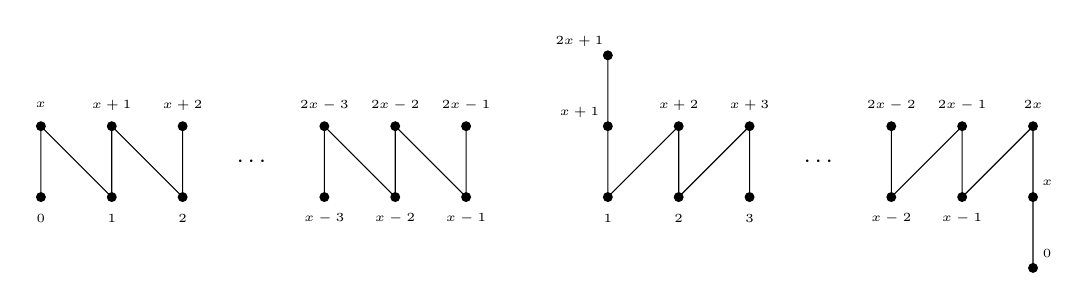
\begin{tikzpicture}[scale=0.9, every node/.style={transform shape}]

\fill (0,1) circle (2pt) ;
\fill (1,1) circle (2pt) ;
\fill (2,1) circle (2pt) ;
\fill (4,1) circle (2pt) ;
\fill (5,1) circle (2pt) ;
\fill (6,1) circle (2pt) ;

\fill (0,2) circle (2pt) ;
\fill (1,2) circle (2pt) ;
\fill (2,2) circle (2pt) ;
\fill (4,2) circle (2pt) ;
\fill (5,2) circle (2pt) ;
\fill (6,2) circle (2pt) ;

\draw (0,1) -- (0,2) -- (1,1) -- (1,2) -- (2,1) -- (2,2) ;
\draw (4,1) -- (4,2) -- (5,1) -- (5,2) -- (6,1) -- (6,2) ;

\node at (0, 0.7) {\tiny 0} ;           
\node at (1, 0.7) {\tiny 1} ;
\node at (2, 0.7) {\tiny 2} ;  
\node at (4, 0.7) {\tiny $x-3$} ;  
\node at (5, 0.7) {\tiny $x-2$} ;  
\node at (6, 0.7) {\tiny $x-1$} ;  

\node at (0, 2.3) {\tiny $x$} ;   
\node at (1, 2.3) {\tiny $x+1$} ;           
\node at (2, 2.3) {\tiny $x+2$} ;
\node at (4, 2.3) {\tiny $2x-3$} ;  
\node at (5, 2.3) {\tiny $2x-2$} ;  
\node at (6, 2.3) {\tiny $2x-1$} ;  

\node at (3, 1.5) {$\cdots$} ;


\fill (8,3) circle (2pt) ;
\fill (8,2) circle (2pt) ;
\fill (8,1) circle (2pt) ;
\fill (9,1) circle (2pt) ;
\fill (10,1) circle (2pt) ;
\fill (12,1) circle (2pt) ;
\fill (13,1) circle (2pt) ;


\fill (9,2) circle (2pt) ;
\fill (10,2) circle (2pt) ;
\fill (12,2) circle (2pt) ;
\fill (13,2) circle (2pt) ;
\fill (14,2) circle (2pt) ;
\fill (14,1) circle (2pt) ;
\fill (14,0) circle (2pt) ;

\draw (8,3) -- (8,1) -- (9,2) -- (9,1) -- (10,2) -- (10,1) ;
\draw (12,2) -- (12,1) -- (13,2) -- (13,1) -- (14,2) -- (14,0) ;

\node at (11, 1.5) {$\cdots$} ;

\node at (14.2, 0.2) {\tiny 0} ;
\node at (14.2, 1.2) {\tiny $x$} ;


\node at (8, 0.7) {\tiny 1} ;           
\node at (9, 0.7) {\tiny 2} ;
\node at (10, 0.7) {\tiny 3} ;  
\node at (12, 0.7) {\tiny $x-2$} ;  
\node at (13, 0.7) {\tiny $x-1$} ;  

\node at (7.6, 2.2) {\tiny $x+1$} ;           
\node at (7.6, 3.2) {\tiny $2x+1$} ;

         
\node at (9, 2.3) {\tiny $x+2$} ;
\node at (10, 2.3) {\tiny $x+3$} ;  
\node at (12, 2.3) {\tiny $2x-2$} ;  
\node at (13, 2.3) {\tiny $2x-1$} ;  
\node at (14, 2.3) {\tiny $2x$} ;

\end{tikzpicture}

\end{document}